\chapter{Graphs and networks}

In general, the complex networks - networks of both randomness and structure - studied in this article can be represented by an undirected and unweighed graph:
\begin{equation}
G = (V,E)	
\end{equation}
, where $V$ is the set of vertices (or nodes), and $E$ is the set of edges (or links).

Each edge connects exactly one pair of vertices, and a vertex-pair can be connected by maximally one edge, i.e., multi-connection is not allowed.
Let furthermore $N$ denote the number of vertices $N = |V|$ and $L$ the number of edges $L = |E|$.

For a social network [9], $V$ is a set of persons (or "actors" in sociology parlance) and $E$ is the set of acquaintance ties that links the persons together.
In computer networks $V$ represent the routers or computers and $E$ the channels for computer communication.

\section{Random graph model} % (fold)
\label{sec:random_graph_model}



One of the models of network formation is the original random-graph model.
This model was studied extensively by the Hungarian mathematicians Paul Erd\"os (1913–1996) and Alfr\'ed R\'enyi (1921–1970), and was responsible for a large corpus of research on random graphs
In the random graph model, a graph has $n$ vertices or nodes, and for every pair of nodes $i, j$, an edge exists with probability $p$.
It is usually denoted by $G(n, p)$, and defines a distribution of graphs $P(G)$.
As with other models studied in this thesis, statements made about the model are statements made about the collection of graphs, rather than any specific instance of a graph.

\begin{figure}[tb]
	\centering
	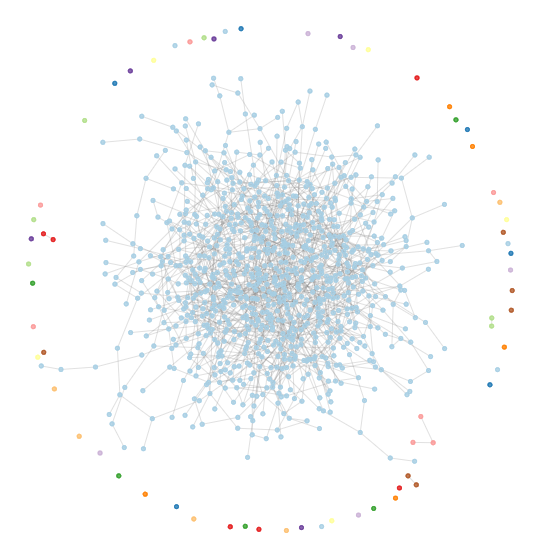
\includegraphics[width=10cm]{figures/gnp_hairball.png}
	\caption{Caption here}
	\label{fig:figure1}
\end{figure}

The random graph model is especially interesting because several of its statistical properties can be derived analytically.
The properties of the networks it generates, however, differ substantially from those observed in real world networks~\cite{Albert:2002p4071}.


\subsection{Mean degree and degree distribution} % (fold)
\label{ssub:mean_degree_and_degree_distribution}


In the random graph model, the existence of any edge is independent from each other and solely determined by the same probability value $p$.
As such, the probability of a graph with $m$ edges drawn from the $G(n,p)$ model is given by a binomial distribution choosing $m$ edges out of a universe of $\binom{n}{2}$ edges
\begin{equation}
	P(m) = \binom{\binom{n}{2}}{m} p^m (1-p)^{\binom{n}{2}-m}
\end{equation}
Using the binomial theorem, 
\begin{equation}
	\mean{m} = \sum^{\binom{n}{2}}_{m=0} P(m) = \binom{n}{2} p
\end{equation}

In the course of this document, we will be not only interested on the properties of the graph itself, but also on how they build from the individual properties of the edges and nodes.
Under the $G(n,m)$ model, the mean degree of the vertices is given by
\begin{equation}
	\mean{k} = \sum^{\binom{n}{2}}_{m=0} \frac{2m}{n} P(m) = \frac{2}{n} \binom{n}{2} p = (n-1) p,
\end{equation}

More generally, we can not only find the mean, but also the entire distribution of the node degree.
In fact, any node in the graph is connected with independent probability $p$ to any of the remaining $n-1$ nodes in the graph.
Hence, the probability of having a particular degree $k$, i.e. being connected to exactly $k$ other nodes, is $p^k (1-p)^{n-1-k}$.
Given that there are $\binom{n-1}{k}$ possible sets of $k$ vertices, the probability distribution of the node degree is given by
\begin{equation}
	p_k = \binom{n-1}{k} p^k (1-p)^{n-1-k}
\end{equation}
When considering large networks we assume $n$ to be large, so that 
$$\ldots   \textrm{derivation of the limit}$$

\begin{equation}
	p_k = e^{-c} \frac{c^k}{k!}
\end{equation}

% subsection mean_degree_and_degree_distribution (end)Mean degree and degree distribution





\subsection{Giant component} % (fold)
\label{sub:giant_component}

Although very simple, the random graph model possesses one very interesting property: the sudden appearance of the so-called giant component by varying the mean degree $c$.
A giant component is a component whose size is proportional to the size of the network $n$, and its sudden appearance is called a \textit{phase transition}.

We define as $u$ the vertices that do \textbf{not} belong to the giant component.
Then, there is a giant component if and only if $u<1$.

Suppose that, under the $G(n,p)$, vertex $i$ does not belong to the giant component.
Consider another vertex $j$.
Either $i$ and $j$ are not connected with probability $1-p$, or there is an edge between $i$ and $j$ and $j$ also does not belong to the giant component, which has a probability of $pu$.
Therefore, the probability that there is an edge $(i,j)$ is $1-p + pu$.
If we now consider every nodes in the graph, then the probability that node $i$ is not in the giant component is $u$, and depends on it only being connected to nodes not being in the giant component.
Since every edge in the graph exists independently, then we have
\begin{equation}
	u = (1- p + pu)^{n-1} = \left[ 1 - \frac{c}{n-1} (1-u)\right]^{n-1}
\end{equation}
If we take the logarithm of both sides, 
\begin{equation}
	\ln u = \ln\left[ 1 - \frac{c}{n-1} (1-u)\right]^{n-1} = (n-1) \ln\left( 1-\frac{c}{n-1} (1-u)\right)
\end{equation}
When $n$ is large, $\frac{c}{n-1}$ is very small, so that we following approximation holds
\begin{equation}
	\ln\left( 1-\frac{c}{n-1} (1-u)\right) \approx - \frac{c}{n-1} (1-u)
\end{equation}

and therefore,
\begin{equation}
	\ln u \approx - c (1-u)
\end{equation}
By taking the exponential of both sides, we can write it as
\begin{equation}
	u \approx e^{-c(1-u)}
\end{equation}
Alternatively, one can consider the reciprocal of $u$, i.e. the fraction $S$ of nodes that do belong to the giant component.
\begin{equation}
	S = 1 - e^{-cS}
\end{equation}
\begin{equation}
	c = - \frac{\ln(1-S)}{S}
\end{equation}
\noindent which is expressed through the Lambert $W$-function
\begin{equation}
S = 1 + \frac{W(-c e^{-c})}{c}
\label{eq:s_giant_component_lambert}
\end{equation}


\begin{figure}[tb]
	\centering
	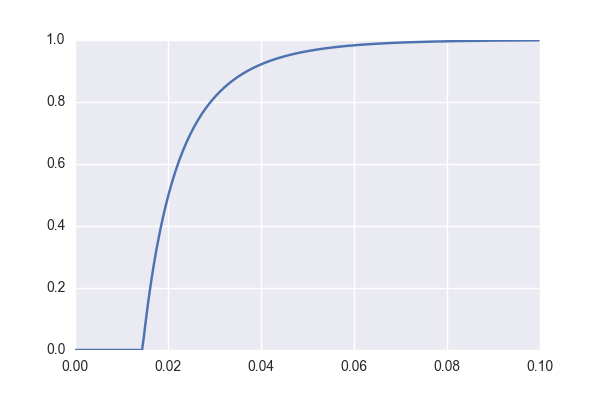
\includegraphics[]{figures/s_as_function_of_p.png}
	\caption{Caption here}
	\label{fig:figure1}
\end{figure}

% subsection giant_component (end)








\subsection{Component sizes} % (fold)
\label{sub:component_sizes}


Generating functions.

The average size of $\mean{s}$ becomes 
\begin{equation}
	\mean{s} = \frac{1}{1-c-cS}
\end{equation}
with $S$ being the fractional size of the giant component, as given by equation~\ref{eq:s_giant_component_lambert}.

% subsection component_sizes (end)


% section random_graph_model (end)

\section{Configuration model} % (fold)
\label{sec:configuration_model}

The configuration model is one of the most popular null models for the study of the statistical properties of networks.
It is inspired 

% section configuration_model (end){Configuration model}

\section{Generating functions} % (fold)
\label{sec:generating_functions}



We assume throughout this chapter that  follow~\cite{Newman:zFi032Kd}, which defines a set of generating functions for the probability distributions of some of the statistical properties of the graphs.
The basis of these is the function $G_0(x)$ for the probability distribution of vertex degrees $k$, defined as
\begin{equation}
G_0(x) = \sum_{k=0}^{\infty} p_k x^k
\end{equation}
where $p_k$ is the probability that a given vertex of the graph has degree $k$.

- normalization assumption ($G_0(1) = 1$)
- $G_0(x)$ is finite for all $|x| \le 1$

The derivatives of this function can be used to derive other statistical quantities.
For example, one can recover the probability $p_k$ by taking the $k^{th}$ derivative of the $G_0$
\begin{equation}
	p_k = \frac{1}{k!} \frac{d^k G_0}{dx^k} \Big|_{x=0}.
\end{equation}

Furthermore, one can obtain the average degree $z$ of the nodes in a graph 
\begin{equation}
	z = \mean{k} = \sum_k k p_k = G'_0(1)
\end{equation}

The function is given by the polylogarithm function
\begin{equation}
	\poly{n}{z} = \sum_{k=1}^{\infty} \frac{z^k}{k^n}
\end{equation}

\subsubsection{Component sizes} % (fold)
\label{ssub:component_sizes}

$H_1(x)$ follows the recursive condition
\begin{equation}
	H_1(x) = x G_1( H_1(x))
\end{equation}








\begin{equation}
\mean{s} = 1 + \frac{G'_0(1)}{1-G'_1(1)}	
\end{equation}




For a Poisson random graph







For a power law graph, this is given by
\begin{equation}
	G_1(x) = \frac{\poly{\tau-1}{xe^{-1/\kappa}}}{x\poly{\tau-1}{e^{-1/\kappa}}}
\end{equation}
and therefore
\begin{equation}
	G'_1(x) = \frac{\operatorname{Li}_{s - 2} \left(x e^{- 1/\kappa}\right)}
	               {x^{2} \operatorname{Li}_{s - 1}\left(e^{- 1/\kappa}\right)} -
	          \frac{\operatorname{Li}_{s - 1}\left(x e^{- 1/\kappa}\right)}
	               {x^{2} \operatorname{Li}_{s - 1}\left(e^{- 1/\kappa}\right)}
\end{equation}

% subsubsection component_sizes (end)Component sizes
% section generating_functions (end)